\documentclass[a4paper]{llncs}
\usepackage[T1]{fontenc}
\usepackage[utf8]{inputenc}
\usepackage[portuguese]{babel}
\usepackage{lmodern}
\usepackage{booktabs}
\usepackage{tabularx}
\usepackage{graphicx}
\usepackage{xcolor}
\usepackage{fancyvrb}

\renewcommand{\keywordname}{{\bf Palavras-chave:}}
\renewcommand{\andname}{e}
\renewcommand{\lastandname}{\unskip\ e}
% Sem cabeçalhos corridos; apenas o número de página no rodapé.
\pagestyle{plain}
\setlength{\tabcolsep}{4pt}
\newcolumntype{L}[1]{>{\raggedright\arraybackslash}p{#1}}
\newcolumntype{Y}{>{\raggedright\arraybackslash}X}
\setlength{\textfloatsep}{8pt plus 2pt minus 2pt}
\setlength{\floatsep}{6pt plus 2pt minus 2pt}
\setlength{\intextsep}{9pt plus 2pt minus 2pt}
% Excertos de código e de consola.
\DefineVerbatimEnvironment{code}{Verbatim}{fontsize=\scriptsize, frame=single,
  framesep=3pt, samepage=true,
  listparameters={\setlength{\topsep}{4pt}\setlength{\partopsep}{0pt}}, rulecolor=\color{black!40}, xleftmargin=1pt, xrightmargin=1pt}
\graphicspath{{../../results/full/figures/}{figuras/}}

\begin{document}

\title{Implementação de mecanismos de QoS\\ usando VNFs\\{\large Relatório de progresso --- TP3}}

\author{André Miguel Rego Trindade Pinto \and Diogo Fernandes Pinto \and\\ Francisco José Fidalgo Lage}

\institute{Grupo PL11 --- Qualidade de Serviço na Internet,\\ Universidade do Minho, Braga, Portugal\\
\email{\{pg65400, pg65405, pg65407\}@alunos.uminho.pt}}

\maketitle

\begin{abstract}
A cadeia de quatro VNFs proposta está implementada e integrada, cada VNF foi testada
isoladamente e a campanha de experiências prevista já foi corrida. Este
relatório mostra excertos do código, capturas do sistema em funcionamento, os
resultados iniciais e o que falta fazer.
\keywords{QoS \and NFV \and VNF \and DiffServ \and Cadeia de serviço}
\end{abstract}

\section{Ponto de situação}

O código, a configuração e os resultados estão no repositório Git do grupo:
\texttt{https://github.com/Daydream127/Qosi}. A Tabela~\ref{tab:estado} compara o
plano da proposta com o estado atual. As Fases~1 e~2 estão concluídas e a Fase~3 está
adiantada em relação ao plano: a cadeia está integrada e a campanha de experiências
já foi corrida.

\begin{table}[!ht]
\caption{Estado do trabalho face ao plano da proposta.}
\label{tab:estado}
\centering
\footnotesize
\begin{tabularx}{\textwidth}{@{}L{3.5cm} Y L{1.5cm}@{}}
\toprule
Fase & O que está feito & Estado \\
\midrule
1 Ambiente e plano & Ubuntu~22.04 com Containernet, Docker e Open~vSwitch,
  instalado por \emph{scripts}. & Concluída \\
2 VNFs isoladas & Quatro VNFs em imagens Docker, gerador de tráfego e
  26~testes automáticos. & Concluída \\
3 Integração e otimização & Cadeia integrada com cinco perfis; campanha de dez
  cenários; otimização iniciada. & Em curso \\
4 Análise e relatório & Campanha completa corrida; gráficos e tabela-resumo
  automáticos. Falta a análise final e o relatório. & Em curso \\
\bottomrule
\end{tabularx}
\end{table}

Há um desvio em relação à proposta. A máquina virtual VirtualBox prevista ficava
demasiado lenta nos computadores do grupo, que têm o Hyper-V ativo, e as medições de
atraso deixavam de ser fiáveis. O ambiente passou a ser uma distribuição Ubuntu~22.04
dedicada no WSL2, instalada pelos mesmos \emph{scripts}; a alternativa com Vagrant e
VirtualBox continua no repositório.

\section{Implementação}

\subsubsection{Topologia e orquestração.}
O orquestrador (\texttt{topology/qosnet.py}) lê a configuração em
\texttt{config/chain.yaml}, cria com o Containernet os contentores e as ligações,
atribui endereços e rotas estáticas e corre em cada VNF o \emph{script}
\texttt{/vnf/start}, com os parâmetros passados em variáveis de ambiente. Cada VNF é um salto IP. A ordem da cadeia é a da
lista no ficheiro de configuração, cujo excerto seguinte mostra a VNF3 e dois dos
perfis de teste:

\begin{code}
chain:
  - name: vnf3
    image: qosi/qos
    env: {LINK_RATE: 10mbit, QUEUE_PKTS: 100, EF_RATE: 1mbit, AF_RATE: 5mbit,
          BE_RATE: 4mbit, EF_POLICE_RATE: 200kbit, AF_POLICE_RATE: 5mbit}
profiles:
  baseline:   {vnf1: {ENABLED: 0}, vnf2: {ENABLED: 0}, vnf3: {SCHEDULING: 0, POLICING: 0}}
  sched:      {vnf2: {ENABLED: 0}, vnf3: {SCHEDULING: 1, POLICING: 0}}
\end{code}

Um perfil só altera variáveis e volta a correr os \emph{scripts} \texttt{start}; uma
VNF desativada fica em modo de passagem. Assim, as configurações com e sem QoS são
comparadas sobre a mesma topologia, sem a reconstruir.

\subsubsection{VNF1 Classificador e VNF2 Firewall.}
As duas usam \texttt{nftables}. O classificador marca o DSCP no gancho
\texttt{forward}: EF para VoIP, AF31 para vídeo e CS0 para o resto, porque na fronteira
de um domínio DiffServ não se confia na marcação feita pelos clientes. A firewall tem
política \emph{default-deny} e só admite os clientes e os serviços autorizados:

\begin{code}
# VNF1 (vnfs/classifier/start)
chain classify {
  type filter hook forward priority mangle; policy accept;
  ip daddr 10.0.2.0/24 udp dport 5004 counter name voip  ip dscp set ef   accept
  ip daddr 10.0.2.0/24 udp dport 5006 counter name video ip dscp set af31 accept
  counter name other ip dscp set cs0
}
# VNF2 (vnfs/firewall/start)
chain forward {
  type filter hook forward priority filter; policy drop;
  ct state established,related counter name allowed accept
  ip saddr @clients ip daddr 10.0.2.0/24 udp dport { 5004, 5006, 5008 }
                                                   counter name allowed accept
  ip saddr @clients ip daddr 10.0.2.0/24 tcp dport { 5201 } counter name allowed accept
  counter name dropped drop
}
\end{code}

\subsubsection{VNF3 Policer/Scheduler.}
A interface de saída da VNF3 é o gargalo de 10~Mbit/s. O agendamento usa HTB com três
classes: EF tem prioridade máxima e fica limitada a 1~Mbit/s, para não esgotar as
outras; AF31 e BE têm débitos garantidos de 5 e 4~Mbit/s e podem usar a capacidade
que sobrar. A marcação segue o RFC~4594~\cite{rfc4594}. O policiamento é feito à entrada, com um \emph{token bucket} por classe que
descarta o tráfego fora do perfil contratado:

\begin{code}
# Agendamento à saída (vnfs/qos/start)
tc qdisc add dev $OUT_IF root handle 1: htb default 30
tc class add dev $OUT_IF parent 1:  classid 1:1  htb rate $LINK_RATE ceil $LINK_RATE
tc class add dev $OUT_IF parent 1:1 classid 1:10 htb rate $EF_RATE ceil $EF_RATE   prio 0
tc class add dev $OUT_IF parent 1:1 classid 1:20 htb rate $AF_RATE ceil $LINK_RATE prio 1
tc class add dev $OUT_IF parent 1:1 classid 1:30 htb rate $BE_RATE ceil $LINK_RATE prio 2
tc filter add dev $OUT_IF parent 1: protocol ip u32 match ip dsfield 0xb8 0xfc flowid 1:10
tc filter add dev $OUT_IF parent 1: protocol ip u32 match ip dsfield 0x68 0xfc flowid 1:20
# Policiamento à entrada
tc qdisc add dev $IN_IF handle ffff: ingress
tc filter add dev $IN_IF parent ffff: protocol ip u32 match ip dsfield 0xb8 0xfc \
   action police rate $EF_POLICE_RATE burst $EF_POLICE_BURST conform-exceed drop
\end{code}

\subsubsection{VNF4 Monitor e medição.}
A monitorização tem duas partes. A passiva conta pacotes e \emph{bytes} por classe DSCP
na VNF4, com contadores do \texttt{nftables}; um exportador em Python, presente em
todas as VNFs, publica esses contadores e as estatísticas do \texttt{tc} (ocupação das
filas e descartes) na rede de gestão. O Prometheus recolhe-os de segundo a segundo e o
Grafana mostra-os num \emph{dashboard} (Fig.~\ref{fig:grafana}). A ativa é feita pelo
gerador \texttt{udpgen}: cada pacote leva um número de sequência e o instante de envio,
e o recetor calcula o atraso num sentido (IPTD), a sua variação (IPDV), as perdas (IPLR)
e o débito. Os contentores partilham o relógio monotónico da máquina, pelo que não há
erro de sincronização.

\begin{figure}[!t]
\centering
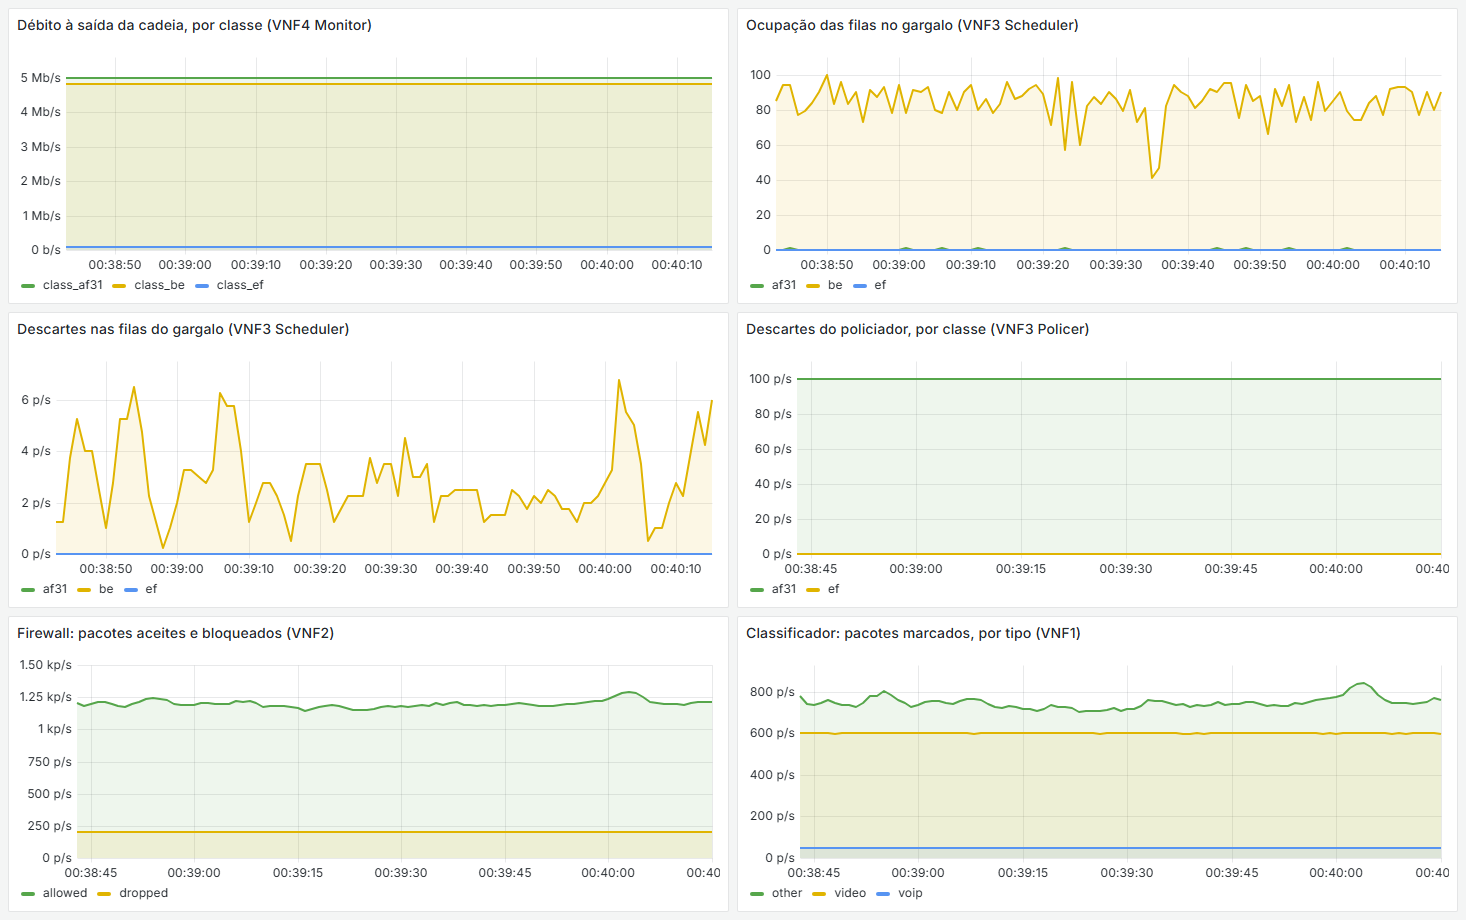
\includegraphics[width=0.93\textwidth]{grafana.png}
\caption{Captura do \emph{dashboard} do Grafana com a cadeia completa, vídeo a
6~Mbit/s (acima do perfil de 5~Mbit/s) e tráfego não autorizado de h\_x.}
\label{fig:grafana}
\end{figure}

\section{Testes e resultados iniciais}

\subsubsection{Testes de cada VNF.}
O comando \texttt{make test} levanta a topologia, ativa uma VNF de cada vez e verifica
o seu efeito com tráfego controlado. A captura seguinte mostra o resultado, com
algumas linhas omitidas:

\begin{code}
$ sudo make test
=== Cadeia em modo de passagem: conectividade e ordem dos saltos
  [OK] traceroute passa por vnf1, vnf2, vnf3, vnf4 e r1
       (10.0.1.1 > 10.0.10.2 > 10.0.11.2 > 10.0.12.2 > 10.0.13.2 > 10.0.2.11)
=== VNF1 Classificador: marcação DSCP
  [OK] VoIP (UDP 5004) marcado como EF  (tos 0xb8)
  [OK] tráfego pré-marcado pelo cliente é remarcado como BE  (tos 0x0)
=== VNF2 Firewall: controlo de acesso
  [OK] h_x: UDP bloqueado  (0 pacotes recebidos)
=== VNF3 Policer: token bucket por classe (EF contratado a 200 kbit/s)
  [OK] VoIP a 400 kbit/s é limitado a cerca de 200 kbit/s  (216.3 kbit/s, perdas 46%)
=== VNF3 Scheduler: congestionamento com e sem agendamento
  sem QoS:  VoIP OWD p95 110.812 ms, perdas 0.20% | vídeo perdas 0.38% | TCP 5834.4 kbit/s
  com HTB:  VoIP OWD p95 5.346 ms, perdas 0.00% | vídeo perdas 0.00% | TCP 5894.8 kbit/s
26/26 verificações passaram
\end{code}

\subsubsection{Campanha de experiências.}
A campanha (\texttt{make experiments}) corre dez cenários, que variam a carga, o
débito do vídeo, o tráfego não autorizado, as condições da ligação ao núcleo e os
parâmetros das filas. Os resultados seguintes são da campanha prevista na proposta:
420~corridas de 60~s, com cinco repetições por ponto. O débito TCP inclui cerca de
2~s iniciais sem tráfego UDP e está sobrestimado em 0,1 a 0,3~Mbit/s. A análise
completa fica para o relatório final.

\begin{table}[!ht]
\caption{VoIP e vídeo em concorrência com quatro fluxos TCP no gargalo de 10~Mbit/s
(médias de cinco corridas).}
\label{tab:carga}
\centering
\footnotesize
\begin{tabularx}{\textwidth}{@{}Y r r r r r@{}}
\toprule
 & \multicolumn{3}{c}{VoIP} & Vídeo & TCP \\
\cmidrule(lr){2-4}
Configuração & IPTD p95 & IPDV & IPLR & IPLR & Débito \\
\midrule
Sem QoS & 108,8 ms & 5,61 ms & 0,52\% & 0,35\% & 5,66 Mbit/s \\
Classificação e agendamento & 5,3 ms & 0,08 ms & 0\% & 0\% & 5,49 Mbit/s \\
Com policiamento & 5,4 ms & 0,10 ms & 0\% & 0\% & 5,37 Mbit/s \\
Cadeia completa & 5,4 ms & 0,09 ms & 0\% & 0\% & 5,43 Mbit/s \\
\bottomrule
\end{tabularx}
\end{table}

Sem QoS, a fila única do gargalo enche com tráfego TCP e o atraso do VoIP passa o
objetivo de 100~ms da classe~0 da Y.1541~\cite{y1541} (Tabela~\ref{tab:carga}). Com classificação e
agendamento, o atraso do VoIP fica reduzido ao atraso do núcleo (5~ms) e deixa de haver
perdas em VoIP e vídeo, com um custo pequeno no débito TCP.

\begin{figure}[!ht]
\centering
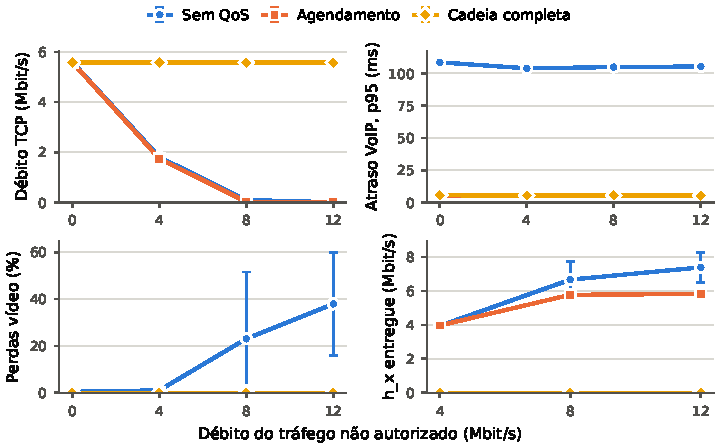
\includegraphics[width=0.9\textwidth]{flood.pdf}
\caption{Efeito de tráfego UDP não autorizado, enviado por h\_x. As barras de erro são
intervalos de confiança de 95\%.}
\label{fig:flood}
\end{figure}

O tráfego não autorizado (Fig.~\ref{fig:flood}) mostra o papel de cada VNF. O
agendamento protege o VoIP e o vídeo, mas o tráfego de h\_x continua a competir com o
TCP na classe \emph{best effort}; só com a firewall o débito TCP se mantém perto de
5,5~Mbit/s. Sem QoS, com 12~Mbit/s de tráfego não autorizado, o VoIP perde 61\% dos
pacotes e o MOS estimado pelo modelo~E simplificado~\cite{cole} desce de 4,3 para 1,3.

Dos restantes cenários, três resultados já são claros. Quando a fonte de vídeo envia
12~Mbit/s, o policiador limita-a a 5~Mbit/s e o TCP mantém 4,5~Mbit/s; sem QoS, o TCP
fica com 0,3~Mbit/s e o VoIP perde 52\% dos pacotes. Filas maiores não dão mais débito
ao TCP, mas aumentam o atraso da classe \emph{best effort} (p95 de 44~ms com 20~pacotes
e de 592~ms com 300). Quanto à sobrecarga, sem o limite de 10~Mbit/s a cadeia encaminha
cerca de 2,8~Gbit/s, contra 8,7~Gbit/s em encaminhamento direto, e acrescenta menos de
0,05~ms de atraso.

\section{Dificuldades e próximos passos}

Além da troca de ambiente, houve duas dificuldades. A primeira versão do gerador usava
o relógio de parede, que o WSL2 acerta com saltos, o que falseava atrasos e débitos em
corridas longas; passou a usar o relógio monotónico. O \texttt{tc} do Ubuntu~22.04 não
produz JSON válido para as classes HTB, e o exportador lê a saída em texto.

Até à entrega final falta: (i)~concluir a otimização, com a escolha fundamentada
do tamanho das filas, dos pesos e dos \emph{token buckets}; (ii)~analisar os cenários
de atraso, perdas e falha no núcleo; (iii)~escrever o relatório final e preparar a
demonstração.

\begin{thebibliography}{[3}
\makeatletter\renewcommand\@biblabel[1]{[#1]}\makeatother  % etiquetas [n], como no estilo IEEE
\bibitem{rfc4594} J. Babiarz, K. Chan, and F. Baker, ``Configuration guidelines for DiffServ service classes,'' RFC 4594, IETF, 2006.
\bibitem{y1541} ITU-T, ``Network performance objectives for IP-based services,'' Rec. Y.1541, 2011.
\bibitem{cole} R. G. Cole and J. H. Rosenbluth, ``Voice over IP performance monitoring,'' \emph{ACM SIGCOMM Comput. Commun. Rev.}, vol. 31, no. 2, pp. 9--24, 2001.
\end{thebibliography}

\end{document}
